\documentclass{article}
\usepackage{graphicx}
\usepackage[brazilian]{babel}
\usepackage[utf8]{inputenc}
\usepackage[T1]{fontenc}
\usepackage{amsmath}
\usepackage{amssymb}
\setlength{\parindent}{0in}

\begin{document}
	
	\title{Lista 2 - Otimização Não Linear}
	\author{Daniel Yoshio Hotta – 9922700}
	
	\maketitle	
	
	\textbf {E7} 
	\\ \\
	
	\textbf {E7.a} 
	\\ \\
	\textit {Resposta:} \\
    
    
    \begin{figure}[h]
    	\caption{Exercício 8.a}
    	\centering % para centralizarmos a figura
    	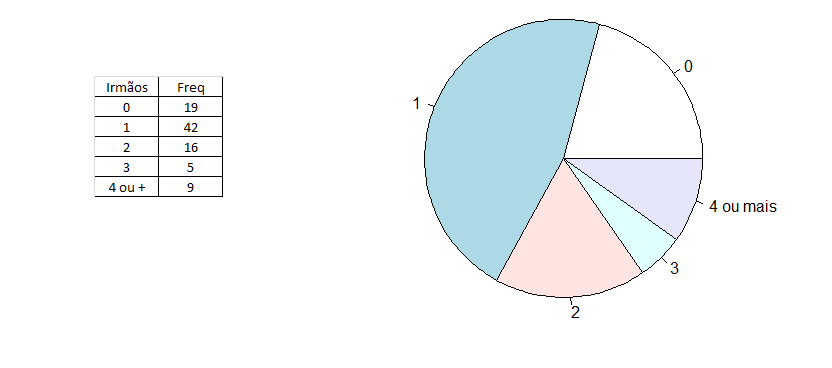
\includegraphics[width=14cm]{8a.png} % leia abaixo
    	\label{figura: Item A}
	\end{figure}
    
    Proporção de 3 ou mais é 14/91.\\
    
    \textbf {E8.b} 
    \\ \\
    \textit {Resposta:} \\
    
    
    \begin{figure}[h]
    	\caption{Exercício 8.b}
    	\centering % para centralizarmos a figura
    	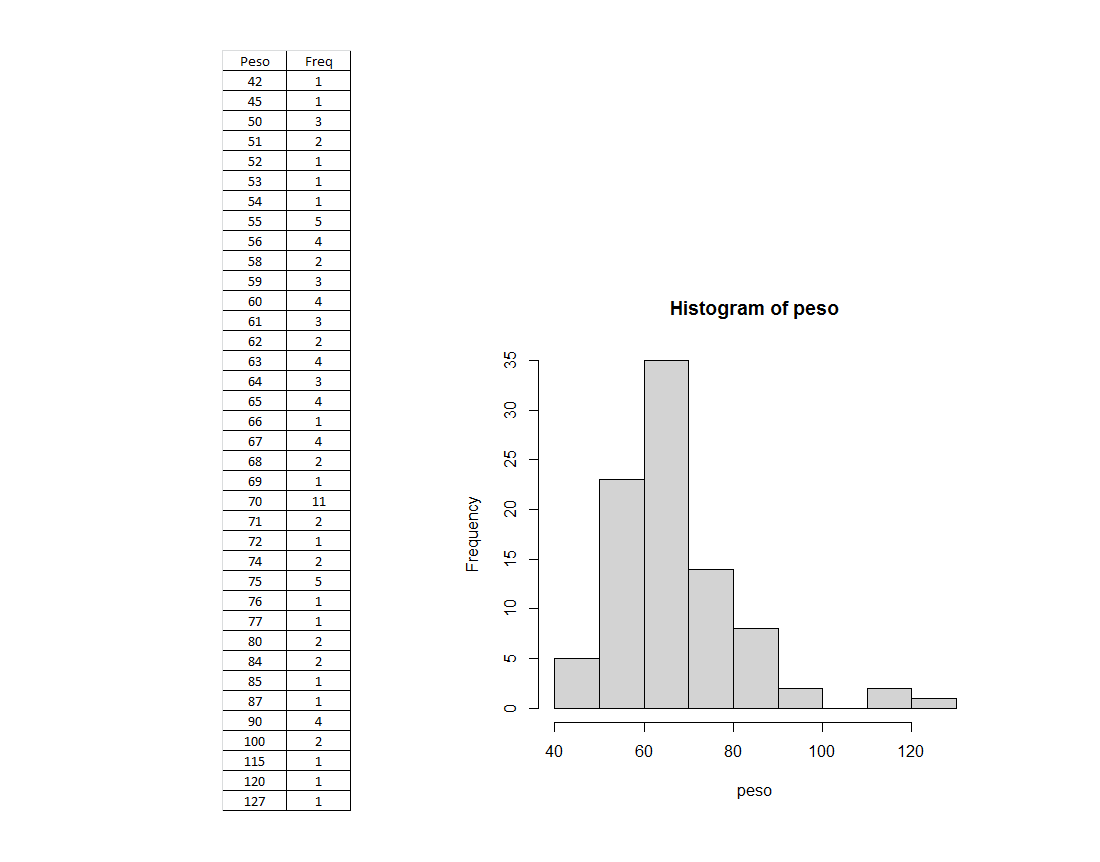
\includegraphics[width=14cm]{8b.png} % leia abaixo
    	\label{figura: Item B}
    \end{figure}

    Lembra o formato de sino, contudo, ainda é um pouco esparso.
	
	\textbf {E8.c} 
	\\ \\
	\textit {Resposta:} \\
	
	
	\begin{figure}[h]
		\caption{Exercício 8.c}
		\centering % para centralizarmos a figura
		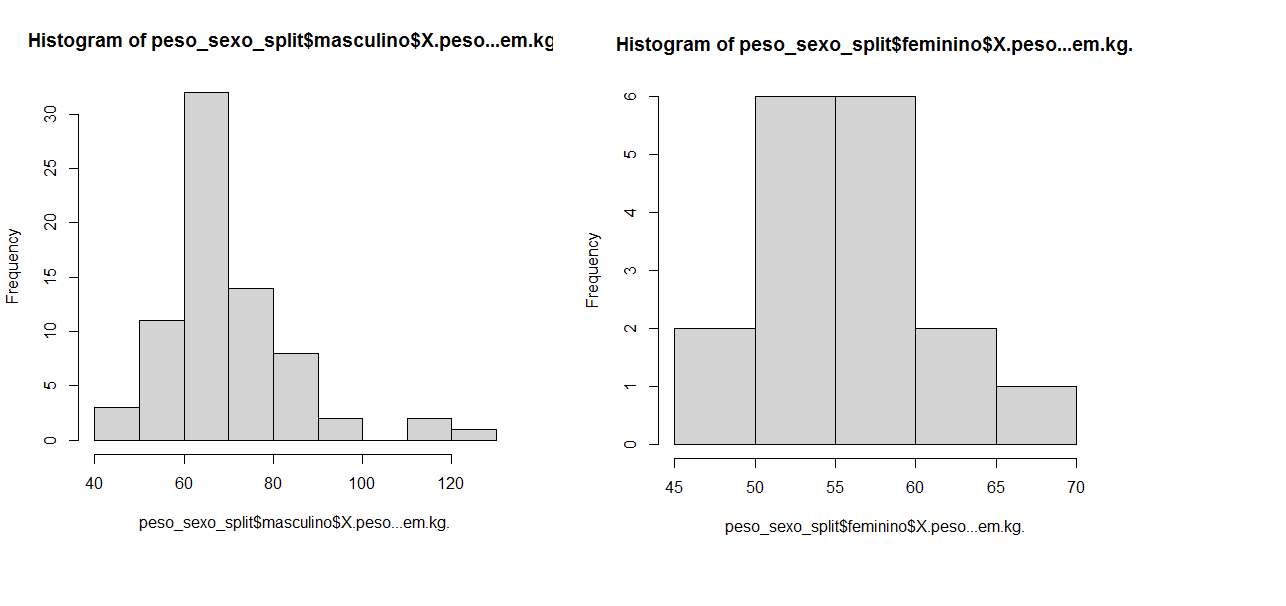
\includegraphics[width=14cm]{8c.png} % leia abaixo
		\label{figura: Item C}
	\end{figure}
	
	
\end{document}
